%-*- coding: utf-8 -*-
\textcolor[RGB]{46, 116, 181}{\chapter{Élaboration}}
\section{Planification des activités}
Nous fixons la date de livraison à 2 semaines avant la présentation. La présentation du projet étant prévue pour le 14/09/2017; notre date de livraison est donc le \textbf{31/08/2017}. Entre le 4 mars et le 31 août, il y a 181 jours moins 7 jours fériés, nous disposons donc de \textbf{174 jours}.

Nous avons identifié huit étapes de développement:
\begin{itemize}
\item Analyse des exigences
\item Cas d'utilisation
\item Modèle de domaine.
\item Séquences système
\item Classes participantes.
\item Diagramme d'intéractions.
\item Classes de conception.
\item Code.
\end{itemize}
Pour évaluer la part de chaque étapes de développement, nous nous basons sur l'affirmation suivante \enquote{Aujourd'hui, un projet c'est 80\% de réflexion et 20\% de développement} (voir \url{http://www.logadap.fr/methodologie-creation-logiciel/}). Ainsi, le code va occuper 20\% de notre temps, soit 35 jours; reste 139 jours à répartir entre les 7 étapes précédentes, soit 20 jours chacunes.
Le diagramme de GANTT est donc le suivant:
\begin{figure}[H]
\label{Gantt}
  \centering
      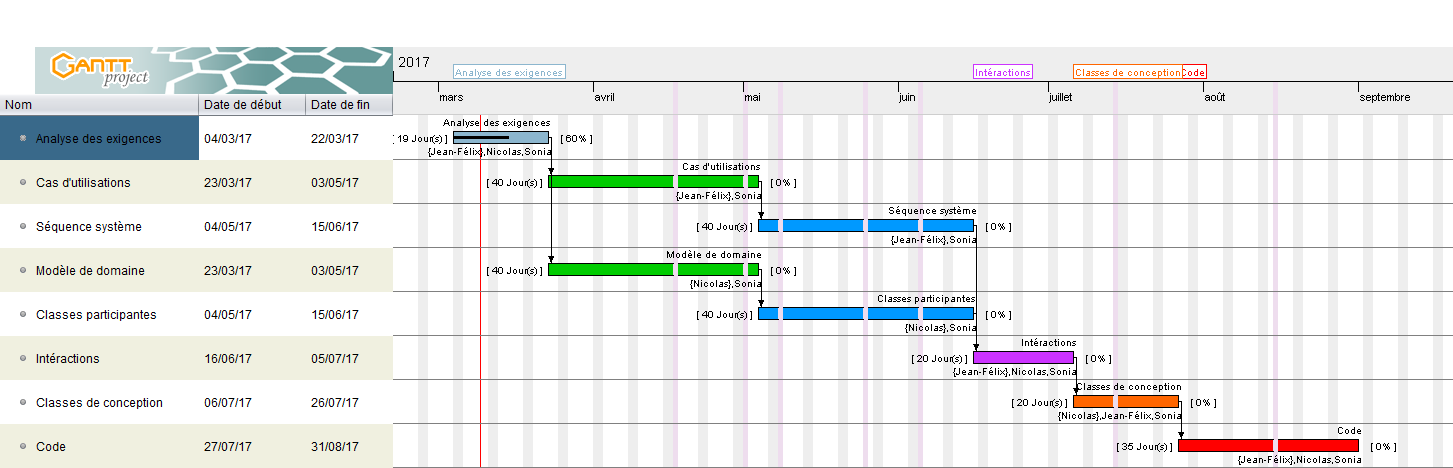
\includegraphics[width=1.0\textwidth]{Vitameal_gantt} %
\caption{Gantt}
\end{figure}

Le diagramme de PERT donne une autre vues de la répartition et de l'enchaînement des taches:
\begin{figure}[H]
\textbf{P}rogram \textbf{E}valuation and \textbf{R}eview \textbf{T}echnique
\label{PERT}
  \centering
      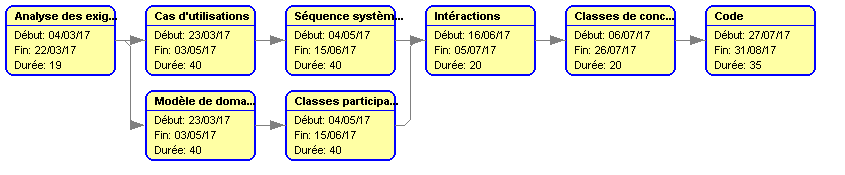
\includegraphics[width=1.0\textwidth]{Vitameal_pert} %
\caption{PERT}
\end{figure}

\section{Affectation des ressources}
Les ressources sont affectées comme suit:

\begin{tabular}{|l|l|}
\hiderowcolors
  \hline
  Tâches & Ressources \\ \hline
  Analyse des exigences & Nicola, Sonia, Jean-Félix \\
  Cas d'utilisation & Jean-Félix 67\%, Sonia 33\% \\
  Modèle de domaine & Nicolas 67\%, Sonia 33\% \\
  Séquences système & Jean-Félix 67\%, Sonia 33\% \\
  Classes participantes & Nicola 67\%, Sonia 33\% \\
  Diagramme d'intéractions & Nicola, Sonia, Jean-Félix \\
  Classes de conception & Nicola, Sonia, Jean-Félix \\
  Code & Nicola, Sonia, Jean-Félix \\ \hline
\end{tabular}

\begin{figure}[H]
\label{Ressources}
  \centering
      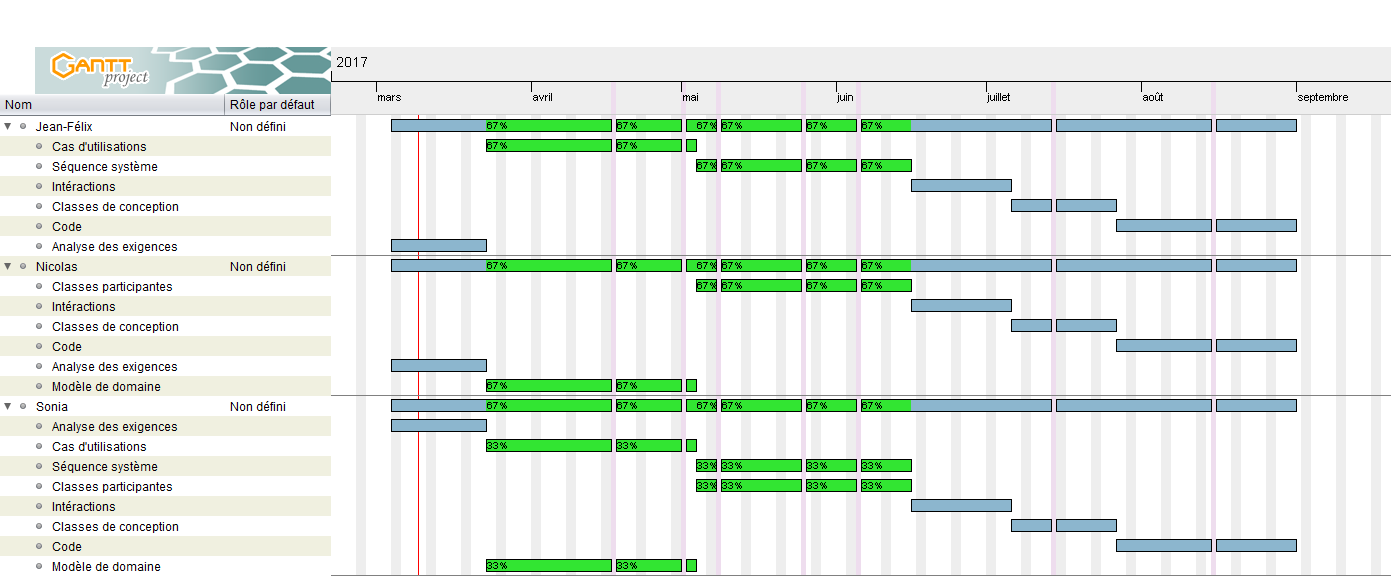
\includegraphics[width=1.0\textwidth]{Vitameal_ressources} %
\caption{Ressources}
\end{figure}

\section{\colorbox{yellow}{TODO} Analyse}

\section{\colorbox{yellow}{TODO} Vision détaillée}

\section{\colorbox{yellow}{TODO} Cible}

\section{\colorbox{yellow}{TODO} Risques}

\section{\colorbox{yellow}{TODO} Besoins précis}

\section{\colorbox{yellow}{TODO} Définition itérative de l'architecture}

\section{\colorbox{yellow}{TODO} Estimation fine}
